\documentclass{article}
\usepackage[utf8x]{inputenc}
\usepackage{ucs}
\usepackage{amsmath} 
\usepackage{amsfonts}
\usepackage{marvosym}
\usepackage{wasysym}
\usepackage{upgreek}
\usepackage[english,russian]{babel}
\usepackage{graphicx}
\usepackage{float}
\usepackage{textcomp}
\usepackage{hyperref}
\usepackage{geometry}
  \geometry{left=2cm}
  \geometry{right=1.5cm}
  \geometry{top=1cm}
  \geometry{bottom=2cm}
\usepackage{tikz}
\usepackage{ccaption}
\usepackage{multicol}

\hypersetup{
   colorlinks=true,
   citecolor=blue,
   linkcolor=black,
   urlcolor=blue
}

\usepackage{listings}
%\setlength{\columnsep}{1.5cm}
%\setlength{\columnseprule}{0.2pt}

\usepackage[absolute]{textpos}

\usepackage{colortbl,graphicx,tikz}
\definecolor{X}{rgb}{.5,.5,.5}


\begin{document}
\pagenumbering{gobble}
\lstset{
  language=C,                % choose the language of the code
  basicstyle=\linespread{1.1}\ttfamily,
  columns=fixed,
  fontadjust=true,
  basewidth=0.5em,
  keywordstyle=\color{blue}\bfseries,
  commentstyle=\color{gray},
  stringstyle=\ttfamily\color{orange!50!black},
  showstringspaces=false,
  numbersep=5pt,
  numberstyle=\tiny\color{black},
  numberfirstline=true,
  stepnumber=1,                   % the step between two line-numbers.        
  numbersep=10pt,                  % how far the line-numbers are from the code
  backgroundcolor=\color{white},  % choose the background color. You must add \usepackage{color}
  showstringspaces=false,         % underline spaces within strings
  captionpos=b,                   % sets the caption-position to bottom
  breaklines=true,                % sets automatic line breaking
  breakatwhitespace=true,         % sets if automatic breaks should only happen at whitespace
  xleftmargin=.2in,
  extendedchars=\true,
  keepspaces = true,
}
\lstset{literate=%
   *{0}{{{\color{red!20!violet}0}}}1
    {1}{{{\color{red!20!violet}1}}}1
    {2}{{{\color{red!20!violet}2}}}1
    {3}{{{\color{red!20!violet}3}}}1
    {4}{{{\color{red!20!violet}4}}}1
    {5}{{{\color{red!20!violet}5}}}1
    {6}{{{\color{red!20!violet}6}}}1
    {7}{{{\color{red!20!violet}7}}}1
    {8}{{{\color{red!20!violet}8}}}1
    {9}{{{\color{red!20!violet}9}}}1
}
\newpage

\title{Семинар \#9: Память. Домашнее задание.\vspace{-5ex}}\date{}\maketitle
\section*{Задачи на работу с памятью}
\textbf{Задача \: 1} Как выглядит память, инициализируемая при создании следующих переменных (в системе с порядком байт Little Endian):
\begin{multicols}{2}
\begin{itemize}
\item \texttt{int a = 0x11223344;}
\item \texttt{int b = 65535;}
\item \texttt{int c = -1;}
\item \texttt{int array[3] = \{10, 2000, 65535}\};
\item \texttt{char str[8] = '{}'Hello'{}'};
\item \texttt{float x = 1.0f};
\item
\begin{verbatim}
struct data {
    char str[5];
    int number;
};
struct data c = {"Cat", 100000};
\end{verbatim}
\end{itemize}
\end{multicols}
Память представить в виде последовательности 2-значных шестнадцатеричных чисел. Например число \\
$123456 = 1e240_{16}$ будет храниться в памяти как \texttt{40 E2 01 00}. \\
\textit{Подсказка:} Чтобы проверить, как будет выглядеть память, можно создать указатель типа \texttt{char*} на эту память и распечатать каждый байт в виде шестнадцатеричного числа:
\begin{lstlisting}
char* p = (char*)&a;
for (int i = 0; i < sizeof(a); ++i) {
    printf("%02x ", p[i]);
}
\end{lstlisting}



\newpage
\section*{Задачи на указатели}
\begin{itemize}

\item \textbf{Указатель на \texttt{int}:} Удвойте значение переменной \texttt{a}, используя только указатель \texttt{p}.
\begin{multicols}{2}
\begin{lstlisting}
#include <stdio.h>
int main() {
    int a = 1234;
    int* p = &a;
    // Тут нужно написать 1 строку кода
    printf("%i\n", a);
}
\end{lstlisting}

\vfill \null    
\columnbreak
\vfill \null 

\begin{center}
\vspace{1cm} 
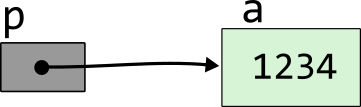
\includegraphics[scale=1]{../images/pointer_schemes/pointer_to_int.png}
\end{center}
\end{multicols}


\item \textbf{Указатель на указатель на \texttt{int}:} Удвойте значение переменной \texttt{a}, используя только указатель \texttt{q}.


\begin{multicols}{2}
\begin{lstlisting}
#include <stdio.h>
int main() {
    int a = 1234;
    int* p = &a;
    int** q = &p;
    // Тут нужно написать 1 строку кода
    printf("%i\n", a);
}
\end{lstlisting}
\columnbreak

\hfill \break
\begin{center}
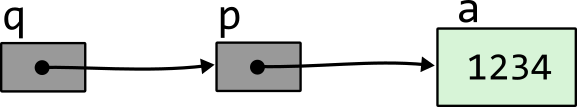
\includegraphics[scale=1]{../images/pointer_schemes/pointer_to_pointer_to_int.png}
\end{center}
\hfill \break

\end{multicols}


\item \textbf{Указатель на элемент массива:} Удвойте значение \texttt{array[1]}, используя только указатель \texttt{p} (не меняя \texttt{p}, он должен указывать на \texttt{array[2]}).
\begin{multicols}{2}
\begin{lstlisting}
#include <stdio.h>
int main() {
    int array[6] = {4, 8, 15, 16, 23, 42};
    int* p = &array[2];
    // Тут нужно написать 1 строку кода
    printf("%i\n", a);
}
\end{lstlisting}
\columnbreak

\hfill \break
\begin{center}
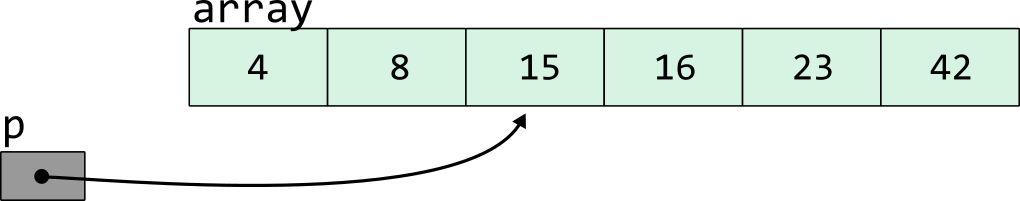
\includegraphics[scale=0.70]{../images/pointer_schemes/pointer_to_array_of_ints.png}
\end{center}
\hfill \break
\end{multicols}

\newpage
\item \textbf{Указатель на структуру} Удвойте значение поля \texttt{year}, используя только указатель \texttt{p}.
\begin{multicols}{2}
\begin{lstlisting}
#include <stdio.h>
struct date {
    int day;
    int month;
    int year;
};
int main() {
    struct date a = {15, 5, 1970};
    struct date* p = &a;
    // Тут нужно написать 1 строку кода
    printf("%d %d %d\n", 
           a.day, a.month, a.year);
}
\end{lstlisting}
\columnbreak

\hfill \break
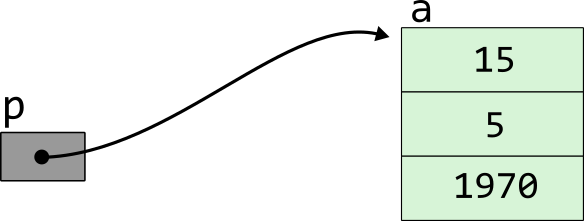
\includegraphics[scale=1]{../images/pointer_schemes/pointer_to_struct_date.png}
\hfill \break

\end{multicols}

\end{itemize}



\subsection*{Указатель на структуру \texttt{Movie}}
\begin{multicols}{2}
\begin{lstlisting}
#include <stdio.h>
struct movie {
    char title[50];
    float rating;
    struct date release_date;
};
typedef struct movie Movie;
\end{lstlisting}
\columnbreak
\begin{center}
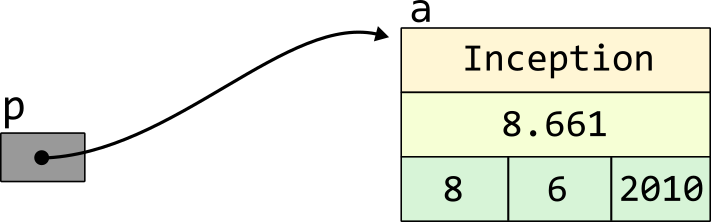
\includegraphics[scale=1]{../images/pointer_schemes/pointer_to_struct_movie.png}
\end{center}
\end{multicols}
\begin{lstlisting}
int main() {
	Movie a = {"Inception", 8.661, {8, 6, 2010}};
	Movie* p = &a;
}
\end{lstlisting}
\textbf{Задача \#12:} Удвойте значение поля \texttt{rating}, используя только указатель \texttt{p}.\\
\textbf{Задача \#13:} Удвойте значение поля месяца выхода фильма, используя только указатель \texttt{p}.

\subsection*{Указатель на массив структур}
\begin{lstlisting}
#include <stdio.h>
struct movie {
	char title[50];
	float rating;
	struct date release_date;
};
typedef struct movie Movie;

int main() {
	Movie a[3] = {{"Inception", 8.661, {8, 6, 2010}}, 
	              {"Green Mile", 9.062, {6, 12, 1999}}, 
	              {"Leon", 8.679, {14, 9, 1994}}};
	Movie* p = &a[1];
}
\end{lstlisting}

\vspace{-59ex}
\begin{center}
\quad\quad\quad\quad\quad\quad\quad\quad\quad\quad\quad\quad\quad\quad\quad\quad\quad\quad\quad\quad\quad\quad\quad
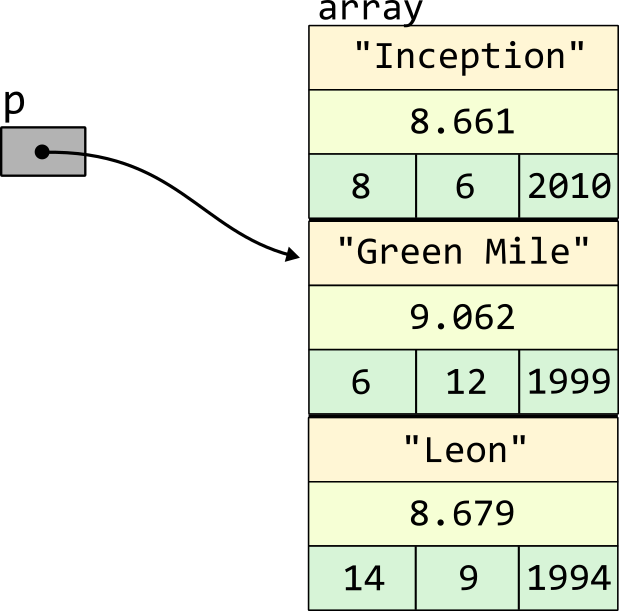
\includegraphics[scale=1]{../images/pointer_schemes/pointer_to_array_of_struct_movie.png}
\end{center}
\textbf{Задача \#14:} Удвойте значение рейтинга фильма \texttt{Inception}, используя только указатель \texttt{p}. (не меняя \texttt{p}, он должен указывать на \texttt{a[1]})\\
\textbf{Задача \#15:} Удвойте значение года выхода фильма \texttt{Leon}, используя только указатель \texttt{p}. (не меняя \texttt{p}, он должен указывать на \texttt{a[1]}).\\


\subsection*{Передача в функцию по значению}
\begin{multicols}{2}
\begin{lstlisting}
#include <stdio.h>

struct movie {
	char title[50];
	float rating;
	struct date release_date;
};
typedef struct movie Movie;

void change_rating(Movie m) {
	m.rating += 1;
}
int main() {
	Movie a = {"Inception", 8.661, 
	             {8, 6, 2010}};
	change_rating(a);
}
\end{lstlisting}
\columnbreak
\begin{center}
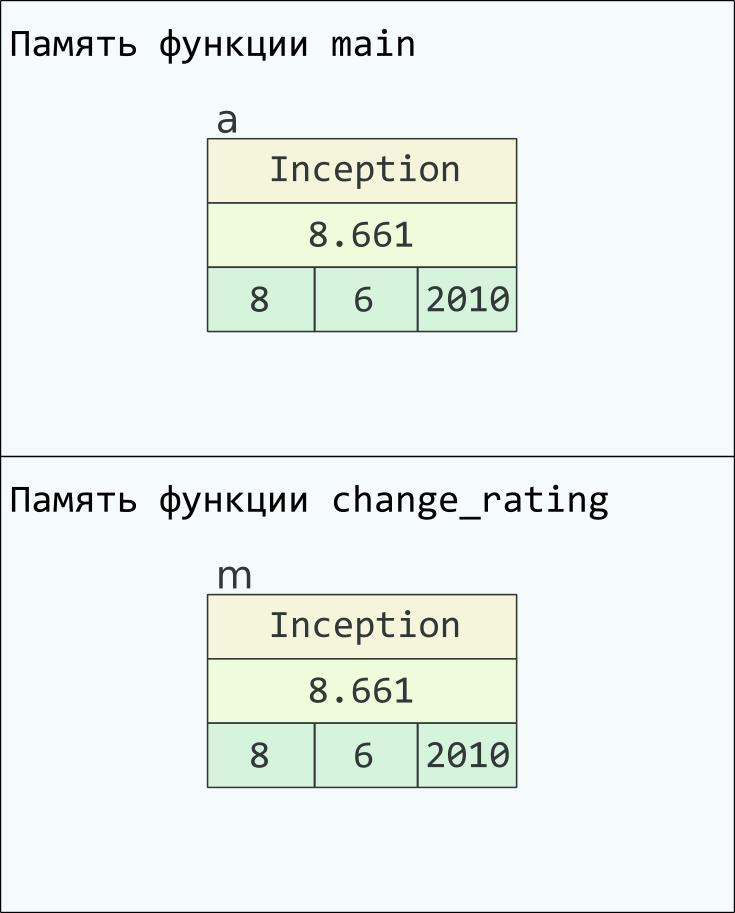
\includegraphics[scale=1]{../images/pointer_schemes/function_by_value.png}
\end{center}
\end{multicols}
Всё, что передаётся в функцию, копируется. Поэтому функция \texttt{change\_rating} будет менять
поле \texttt{rating} у копии структуры \texttt{a}, а изначальная структура не изменится.

\subsection*{Передача в функцию по указателю:}
\begin{multicols}{2}
\begin{lstlisting}
#include <stdio.h>

struct movie {
	char title[50];
	float rating;
	struct date release_date;
};
typedef struct movie Movie;

void change_rating(Movie* pm) {
	pm->rating += 1;
}
int main() {
	Movie a = {"Inception", 8.661, 
	             {8, 6, 2010}};
	Movie* p = &a;
	change_rating(&a);
}
\end{lstlisting}
\columnbreak
\begin{center}
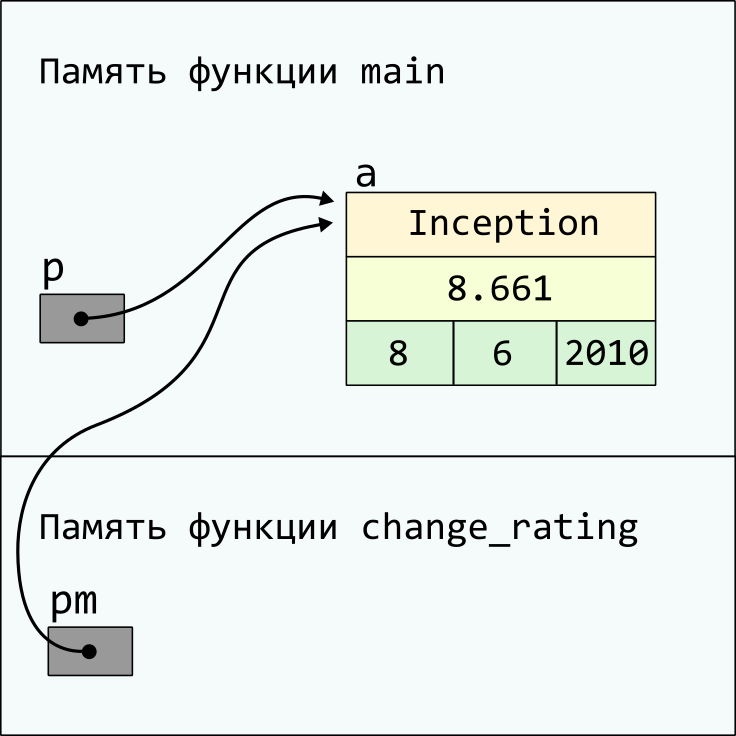
\includegraphics[scale=1]{../images/pointer_schemes/function_by_pointer.png}
\end{center}
\end{multicols}
Всё, что передаётся в функцию, копируется. Но теперь туда копируется указатель, который содержит
адрес стурктуры \texttt{a}. Используя этот указатель, мы можем изменить изначальную структуру. Более того, так как указатель занимает меньше память, его копирования в функцию происходит быстрее, чем копирование всей структуры.\\\\
\textbf{Задача \#16:} Напишите функцию \texttt{change\_day(struct date* pd)}, которая будет увеличивать день на \texttt{1}. Используйте эту функцию, чтобы увеличить день даты выхода на \texttt{1} у структуры \texttt{a}.\\


\end{document}
